\chapter{Implementation}
\label{Implementation}
This chapter describes the implementation details of the system and shows the internal
architecture. All system components are implemented in Typescript that is later compiled to Javascript. This choose of language enables code sharing between individual components and allow us to support multiple platforms (desktop via Node.js, and browser). All system components are dependent on Explorer-core module where is the whole database system implemented (see Figure \ref{systemArchitecture}). 


\begin{figure}[h]
    \centering
    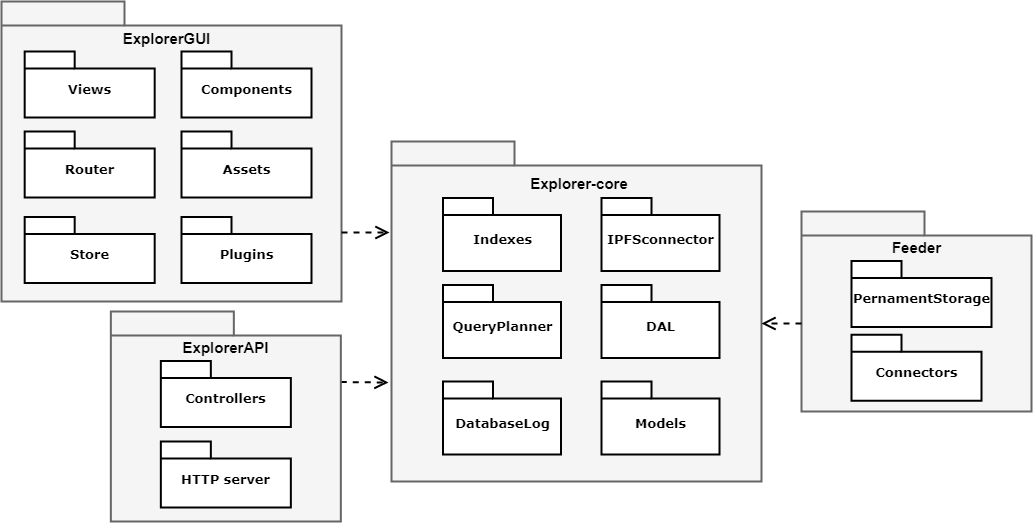
\includegraphics[width=\textwidth]{ExplorerArchitecture.png}
    \caption{System architecture}
    \label{systemArchitecture}
\end{figure}


\section{Explorer-core implementation}
Explorer-core is the most complex module of a whole system with more than 5000 lines of code. The database is a main part of the explorer-core module. Database system consists of a query system, indexes and a database abstract layer. Explorer-core is only system components that communicates with ipfs via js-ipfs\footnote{\url{https://github.com/ipfs/js-ipfs}} implementation.

\subsection{Indexes}
For indexing there is currently implemented only B-tree, but different structures such as tries\footnote{\url{https://en.wikipedia.org/wiki/Trie}} can be implemented easily. They only need to implement index's interface (function such as \texttt{insert}, \texttt{delete}, \texttt{update}, \texttt{find}). We can create indexes on database entities with decorators\footnote{\url{https://www.typescriptlang.org/docs/handbook/decorators.html}}, which are part of ECMAScript 6 standard. Every database entity has to have \texttt{PrimaryKey} decorator on property that is used as a primary index. Index has three parameters:
\begin{itemize}
    \item \texttt{comparator} - is a function that accepts two arguments and returns number that is less than zero if first arguments is greater than second, zero if arguments are the same, more then zero if a second argument is greater than first. If a user has not set any custom comparator default one (\texttt{(a, b) =>
    a < b ? -1 : +(a > b)}) is used. This default comparator works on atomic keys such as string or numbers. 
    \item \texttt{keyGetter} - is another function that accepts a whole entity as arguments and returns key, that is used in an index. A default key getter is function that returns property of the entity (for example default key getter for property \texttt{height} is \texttt{(e) =>  e[''height'']}).
    \item \texttt{branching} - the branching factor is the number of children at each node, the outdegree. Default branching factor is 16.
\end{itemize}

The B-tree structure (see Figure \ref{btree}) is optimized for IPFS. Unlike PostgreSQL B-tree\footnote{\url{https://github.com/postgres/postgres/tree/master/src/backend/access/nbtree}}, leaf nodes have not got left and right sibling references due to cyclic reference this is not possible in IPFS. Cyclic references are not possible, because links are changing CID of an object. Therefore if we store object \texttt{A} with a link to the object \texttt{B}, CID of \texttt{A} will change. Then if we add backlink from \texttt{B} to \texttt{A}, CID of \texttt{B} will be changed and so \texttt{A} has now link to an old version of \texttt{B}. If we update link of object \texttt{A} to point on the new version of object \texttt{B}, CID of object \texttt{A} will change and therefore object \texttt{B} is now pointing to the old version of object \texttt{A}. From this example, it appears that there is no way of making cyclic references in IPFS. Without siblings references we don't have to store data only in leaves, but we can some store data in nodes itself. This approach lead to better performance when executing queries. In insert queries, statistically fewer nodes needs to be updated. Also in search queries, there is a chance that we found a key in some non-leaf node, and therefore we would need fewer node visits.

All search queries (equal, less, greater, between) has two steps:
\begin{itemize}
    \item \textbf{Find subtree} - First, we need to find minimal subtree that contains all results. We start in a root node of the B-tree. Then, we use an index's \texttt{comparator} function to determine if we can visit some child node and still have all the result in it. If not, we found a minimal subtree for the query.
    \item \textbf{Traverse} - To get results of the query we can traverse minimal subtree in two direction. In-order for \texttt{greater than} and \texttt{between}. For \texttt{less than} reversed in-order. With \texttt{equal} it does not matter.
\end{itemize}

\begin{figure}[h]
    \centering
    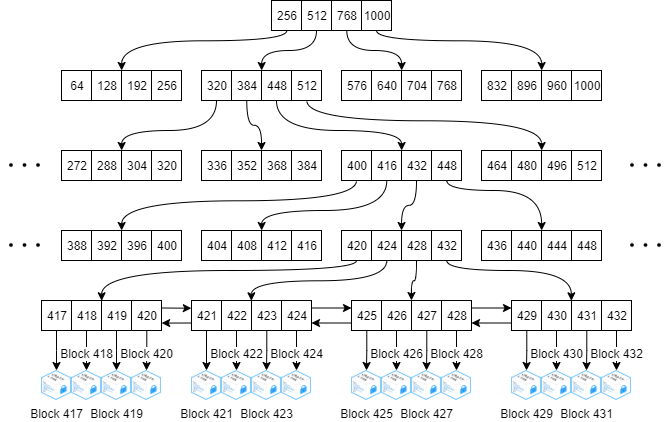
\includegraphics[width=13cm]{btreeindex.png}
    \caption{Btree indexing first 100 blocks by their height}
    \label{btree}
\end{figure}

\subsection{Query system}
Database system offers a complex query system. A query can consist of multiple conditions and the \texttt{Query Planner} is responsible for resolving them. It decides which indexes are used for query and choose a strategy. If there is no condition, a primary key is used for query execution. In the case of a single condition, \texttt{Query Planner} checks if there is an index on the condition's property. If yes, then this index is used to perform the query. Else condition is transformed to filter and a primary key is used to obtain results which are then filtered. For multiple conditions connected with logical operators \texttt{AND} or \texttt{OR}, \texttt{Query Planner} creates \texttt{OR-hashset} and \texttt{AND-hashset}. \texttt{AND-hashset} is initialized with the results of a condition which has the smallest number of results and uses \texttt{AND} operator. Then we check for each result hash for all other \texttt{AND} conditions if \texttt{AND-hashset} contains it. If no, a hash is deleted from \texttt{AND-hashset}. This creates intersection between all \texttt{AND} conditions. The \texttt{OR-hashset} is created empty. Then, we add a hash of every result of all \texttt{OR} conditions to it. This creates union between \texttt{OR} conditions. At the end, we perform union between \texttt{AND-hashset} and \texttt{OR-hashset}. This creates final hashset which is used later to obtain actual data with resolvers such as \texttt{all}, \texttt{first}, \texttt{paginate} etc. If one of the \texttt{AND} conditions has great selectivity (it has less than a hundred results), \texttt{Query Planner} can decide to don't use other indexes, but transform condition to filter and cycle over the results. Example query returning blocks between 38 and 42 is shown in Figure \ref{btreeQuery}. A peer needs to download only data that are highlighted in green. After downloading them, they are stored on peer's filesystem and are offered to other peers. 

\begin{figure}[h]
    \centering
    \includegraphics[width=13cm]{btreeIndexQuery.png}
    \caption{Data access for performing query that returns blocks that have a height between 38 and 42.}
    \label{btreeQuery}
\end{figure}


We can make queries with every database table model (such as model on Figure \ref{classExample}). When object inherits from \texttt{Queriable} class, it gets access to these query methods:
\begin{itemize}
    \item \texttt{where(propertyName)} - create a condition on the property. There can be multiple conditions in one query. A condition hash to be followed by one of the functions: 
    \begin{itemize}
        \item \texttt{gt(value)} - property is greater or equal than \texttt{value}. The QueryPlanner finds in an index first object that has property (set by \texttt{propertyName} in \texttt{where} function) equal or greater than \texttt{value}, and traverse index to the right (to bigger objects).
        \item \texttt{lt(value)} - property is less or equal than \texttt{value}. Similar as in the \texttt{gt} function, the QueryPlanner finds the closest object that has property equal or less than \texttt{value}. Then, the query traverses index to the smaller objects with smaller index value (to the left).
        \item \texttt{between(min, max)} - property is greater or equal than \texttt{min} and less or equal than \texttt{max}. 
        \item \texttt{equal(value)} - returns all objects that \texttt{keyGetter} function returns same key as \texttt{value}. 
    \end{itemize}
    \item \texttt{skip(offsetValue)} - query will skip \texttt{offsetValue} number of results,
    \item \texttt{limit(limitValue)} - set maximum number of results. After query has \texttt{limitValue} count of matched objects it will stop browsing the index,
    \item \texttt{all()} - return all objects that matched query,
    \item \texttt{first()} - return the first object that matched a query,
    \item \texttt{and(childQuery)} - logical and between two queries. Parent query resolves \texttt{childQuery} (call \texttt{all()} function) and add its results to \texttt{AND-hashset}.
    \item \texttt{or(childQuery)} - logical or between two queries. \texttt{childQuery} will be resolved by parent query, and its results stored in \texttt{OR-hashset} of parent query. 
    \item \texttt{[Symbol.iterator]()} - iterator that is used in cycle \texttt{for (result of query)}.
\end{itemize}



\subsection{Database}
The most important part of the Explorer-core module is the database system which connects the query system with indexes. When we make a query, it translates to the database, and data are obtained with a help of the indexes.

\subsubsection{Tables}
A database contains tables that consists of indexes. A table has interface that provide basic CRUD operations on its data:
\begin{itemize}
    \item \texttt{create} - creates history log for entity with first entity version. Then adds it to every table index.
    \item \texttt{update} - adds new version of the entity to its history log. Than update every index of the table.
    \item \texttt{delete} - removes entity from every table index. From now, an entity can not be find in this table.
    \item \texttt{select} - obtain data. If no condition is set, table uses primary key index.
\end{itemize}

Example of the class User is in Figure \ref{classExample}. It has two indexes. One primary on property \texttt{name} and one normal index on property \texttt{age}. The second index has also specified \texttt{comparator} that is a bit faster than default one, but works only on numbers, and \texttt{keygetter} that returns a year when a user has born. 

\begin{figure}[h]
    \centering
    \begin{lstlisting}[style=ES6]
    class User extends Queriable<User> {
        @PrimaryKey()
        name: string;

        @Index(
            (a, b) => a - b,
            u => new Date().getFullYear() - u.age,
        )
        age: number;
    }
    \end{lstlisting}
    \caption{Example of database table abstraction }
    \label{classExample}
\end{figure}



\subsubsection{Transactions}
A database can be executing only a single transaction at the time to prevent data inconsistency. For that reason, we implemented a transaction queue where transactions are stored before executing in the order in which they came. Executing more transactions in a row is significantly more effective than executing them one by one. If a transactions queue has only one transaction, it will wait 100ms for more transactions to come.  

\subsubsection{Synchronization}
There are two types of transactions. Those that changes the database state (\texttt{create}, \texttt{update}, \texttt{delete}) and those that don't (\texttt{select}). Every transaction that changes database state need to be synchronized with other peers. We created Database log for that. It is an append-only log with a discrete-time. There can be only one valid database transaction in every point in time. There are several strategies to choose which transaction is globally accepted and which transactions need to rollbacks (described in design \ref{designSync}).


\todo{popisat algoritmus synchronizacie}


\begin{figure}[h]
    \centering
    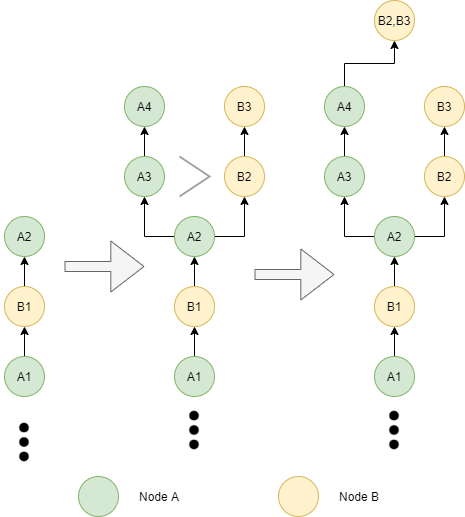
\includegraphics[width=10cm]{syncDB.png}
    \caption{Database synchronization}
    \label{syncDB}
\end{figure}

\section{Feeder}
A Feeder is a simple command-line application written in Typescript (see Algorithm \ref{feederAlgo}). It strongly depends on the Explorer-core module. Currently, we support only Blockbook connector as a source of blockchain's data, but Feeder can be simply expanded to support more data source such as InsightAPI or direct connection to a blockchain as a full node. Each Feeder has configuration file (usually called \texttt{.env}) with Feeder's settings. Main Feeder settings are \texttt{URL} of the source for the blockchain's data and \texttt{DB\_NAME} which is a name of the database where Feeder inserts new blocks. A Feeder can be connected to only one blockchain. We can create multiple Feeders for single blockchain, but we need to provide some deterministic algorithm, that insures that each block is parsed by only one Feeder. This can be done by providing \texttt{FeederId} and \texttt{FeedersCount}  in \texttt{.env} config file. If those values are provided, Feeder parses only blocks that have height modulo \texttt{FeedersCount} equals to \texttt{FeederId}. 


\begin{algorithm}[H]
    \SetAlgoLined
    load configuration\;
     \While{there is new block}{
         fetch block\;
         \For{transaction in block}{
            save transaction\;
            }
          save block\;
     }
    \caption{Simplified Feeder algorithm}
    \label{feederAlgo}
\end{algorithm}


\subsection{ExplorerGUI}
ExplorerGUI is a single page application with a simple user interface implemented with Vue.js\footnote{\url{https://vuejs.org/}} that runs in a browser. We use browser implementation of IndexedDB\footnote{\url{https://developer.mozilla.org/en-US/docs/Web/API/IndexedDB_API}} as a storage for IPFS. Communication with other peers is provided though WebRTC\footnote{\url{https://webrtc.org/}} and WebSockets because a webpage in a browser can not open TCP socket. Every opened ExplorerGUI browser tab is the same IPFS node instance. Opening a new tab in incognito mode or different browser will spawn new IPFS node.

\begin{figure}[h]
    \centering
    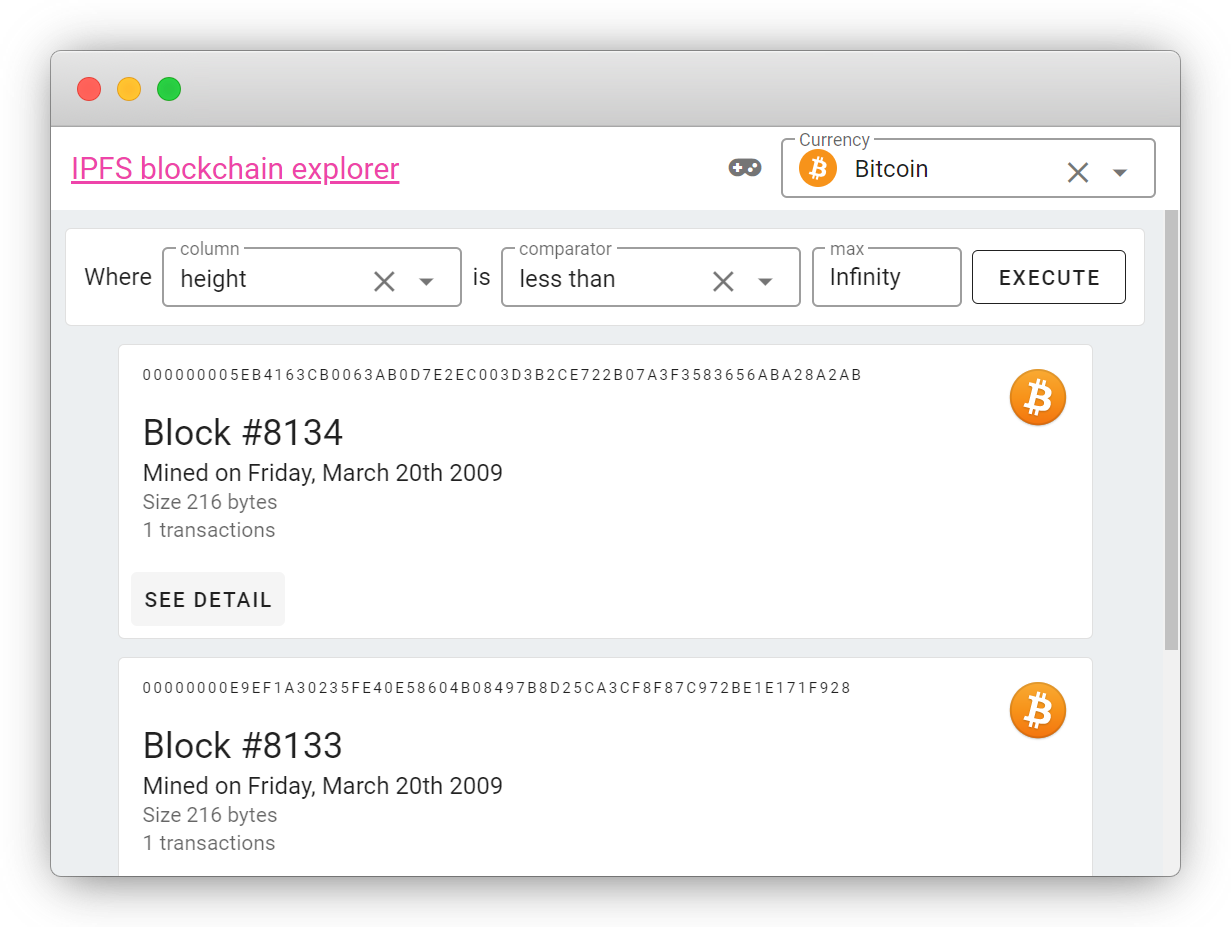
\includegraphics[width=13cm]{blocksView.png}
    \caption{Blocks view}
    \label{blocksView}
\end{figure}

After page with ExplorerGUI is loaded, it tries to connect to all supported blockchains. The home screen contains all enabled cryptocurrencies. Blocks list view is displayed when a user selects specific cryptocurrency. A user can filter blocks by all blocks indexes in this view. A default filter get all blocks that height is less than infinity. This query sorts blocks from the newest (highest) to the oldest (see Figure \ref{blocksView}). When a user clicks on the Execute button, ExplorerGUI starts loading blocks that match the selected query by the asynchronous algorithm shown on Figure \ref{blocksLoading}. First, we use \texttt{iterate} function (implemented in ExplorerCore module) to obtain iterator over subtree of all results. This function is asynchronous, so it does not block the main Javascript thread while it is searching whole index and looking for the subtree. Then we create an array of promises\footnote{\url{https://developer.mozilla.org/en-US/docs/Web/JavaScript/Reference/Global_Objects/Promise}} in which the individual blocks that are displayed on the page are loaded. In for cycle, we push asynchronous tasks to the array. A task contains single parameter that is \texttt{pagePosition}. This parameter is the order of the block that tasks loads. Every task for each block then runs in parallel. First, task call \texttt{next} function on subtree iterator. This function returns the next block in the subtree. \texttt{next} function can return left or right sibling of the current block. It depends on the condition. A subtree is traversed to the left if \texttt{greaterThan} or \texttt{between} condition is used and to the right if there is \texttt{lessThan} condition. \texttt{next} function returns a pair value. \texttt{blockPromise} is a task that loads blockchain block from IPFS and \texttt{done} is boolean, which signals if there are any more results in the subtree. Finally, task waits until blocks is loaded, and then assigns block in the right index of the blocks array. Thanks to this optimized asynchronous algorithm, all blocks that are displayed on the page are loaded in parallel.

\begin{figure}[h]
    \centering
    \begin{lstlisting}[style=ES6]
const subtree = await query.iterate()
const tasks = [];
for (let i = 0; i < pageSize; i++) {
    tasks.push(
        (async pagePosition => {
            const { blockPromise, done } = await subtree.iterator.next();
            if (done)
                return;
            blocks[page - 1 * pageSize + pagePosition] = await blockPromise;
        })(i),
    );
}
await Promise.all(tasks);
    \end{lstlisting}
    \caption{Loading blocks from database}
    \label{blocksLoading}
\end{figure}



\subsection{ExplorerAPI}
Node.js\footnote{\url{https://nodejs.org/}} implementation of IPFS uses filesystem to store data (see Figure \ref{nodeIPFS}). On the top of ExplorerCore, there is a simple web framework Express\footnote{\url{http://expressjs.com/}}, where are routes (endpoints) defined. Currently available routes are described in Section \ref{explorerAPIroutes}. Every route supports query parameters \texttt{filter} (used for filtering results) and \texttt{limit} (which reduces number of results). Pagination can be made by setting \texttt{filter} to be greater/smaller (depending on ordering) as key of the last displayed object and \texttt{limit} to page size. For example, if a user is looking at page of transactions ordered by time (ordered from the newest transactions to the oldest), the next page of transactions are first \(N\) transactions that happened before last displayed transaction (where \(N\) is page size).

Rest API supports optional path param \texttt{path} that is useful for traversing objects in IPFS. If we want to get fifth transaction of the block with height 1000 one of the way is request URL \texttt{/block/998/next\_block/next\_block/txs/5} (get block with height 998, get next block two times, get transaction, a get fifth item from array of transactions). This approach allows the user to explore IPFS storage as graph very quickly by objects links.

